%%%%%%%%%%%%%%%%%%%%%%%%%%%%%%%%%%%%%%%%%%%%%%%%%%%%%%%%%%%%%%%%%%%%%%%%%%%%%%%%%%%%%%%%%%%%%%%%%%%
% Chapter 1 -> Introduction
% Author: Eduardo G Gusmao
%%%%%%%%%%%%%%%%%%%%%%%%%%%%%%%%%%%%%%%%%%%%%%%%%%%%%%%%%%%%%%%%%%%%%%%%%%%%%%%%%%%%%%%%%%%%%%%%%%%
\chapter{Introduction}
\label{cha:introduction}

\graphicspath{{chapter1/figs/}}

%%%%%%%%%%%%%%%%%%%%%%%%%%%%%%%%%%%%%%%%%%%%%%%%%%%%%%%%%%%%%%%%%%%%%
% Section: Motivation
%%%%%%%%%%%%%%%%%%%%%%%%%%%%%%%%%%%%%%%%%%%%%%%%%%%%%%%%%%%%%%%%%%%%%
\section{Motivation}
\label{sec:problem.motivation}

\subsubsection{Gene Regulation and Transcription Factor Binding Sites}

% Genome is not enough
A couple of years ago, it was believed that, in possession of the complete genome for a given organism, it would be possible to exactly determine its phenotype and disease susceptibility. However, after the analysis of the first genomes, it was clear that the simple determination of an organism's DNA nucleotide sequence is not enough to explain the great diversity of biological processes. Such processes are governed by a complex chain of events called ``gene regulation''. Gene regulation includes a wide range of mechanisms that happen inside a cell in which genes are turned ``on'' (i.e. they are expressed) and ``off'' (i.e. they are not expressed) dynamically. Depending on which genes are ``on'' or ``off'', the cell specializes in different functionalities~\citep{maston2006}.

% Post-genomic era
These regulatory mechanisms drive the correct execution of biological processes and require a set of carefully orchestrated steps that depends on the correct spatial and temporal expression of genes~\citep{maston2006}. Therefore, the deregulation of gene expression is often linked to diseases~\citep{encode2012}. In the so-called post-genomic era, attention is turning to the understanding of how protein-coding genes (about $25,000$ in humans) and their products are regulated~\citep{maston2006}.

% Regulatory elements
To understand the molecular mechanisms that dictate the cell's expression patterns, it is important to identify the regulatory elements involved in these activities. One of the most important regulatory features are transcription factors (TFs) -- proteins that bind on the DNA enhancing or repressing the expression of genes. These proteins bind to particular genomic regions called transcription factor binding sites (TFBSs)~\citep{maston2006}. TFBSs may be active if they are currently being bound by a TF or inactive, if they are not currently being bound by a TF. In this thesis, we will address the problem of detecting active TFBSs using a computational approach.

\subsubsection{Computational Detection of Active TFBSs Must Consider the Chromatin Dynamics}

% Sequence-based methods
The first computational approach to identify TFBSs was based solely on the DNA sequence~\citep{stormo2000}. Each TF has a particular DNA sequence affinity, i.e. they tend to bind to specific DNA sequences. The computational sequence-based methods search the genome for DNA substrings that corresponds to target TFs. However, computational sequence-based methods are not able to identify \emph{active} TFBSs, i.e. regions in the genome which are currently being bound by a TF~\citep{pique2011}. This happens because such computational approach does not consider the fact that only a few regions in the genome are accessible for TFs to bind. These regions are called ``open chromatin regions''. The number of open chromatin regions and their location vary between different cell types and ultimately dictates which genes are accessible and being expressed~\citep{encode2012}.

% NGS techniques
Recent advances in biological techniques~\citep{shendure2008} have enabled the creation of experimental methods to identify these open chromatin regions~\citep{encode2012}. We will explore two of these so-called ``open chromatin next-generation sequencing (NGS) techniques'': the chromatin immunoprecipitation followed by NGS -- termed ChIP-seq~\citep{johnson2007}; and the DNase I cleavage followed by NGS -- termed DNase-seq~\citep{crawford2004,sabo2004a}. These techniques generate signals which span the entire genome and indicates open chromatin regions. These signals can be viewed as a vector of numeric values associated to every genomic position. Moreover, certain patterns in the signals generated by DNase-seq and ChIP-seq are indicative of active TFBSs. Therefore, we can apply computational methods to process the DNase-seq and ChIP-seq signals and to identify these patterns. By doing so, we can detect active TFBSs considering the open chromatin information and without the need to use DNA sequence information

\subsubsection{Computational Detection of Active TFBSs Using DNase-seq and ChIP-seq}

% Histone modification ChIP-seq and DNase-seq
The DNA is found wrapped in proteins called histones. There are a number of post-translational modifications on these histones which are indicative of open chromatin regions, such as the so-called H3K4me1 and H3K4me3. By performing a histone modification ChIP-seq experiment we are able to identify cell-specific open chromatin regions. Furthermore, the DNase-seq data also provides a robust map of open chromatin regions with a very high spatial resolution. By combining these two experimental data, we observe very characteristic patterns indicating the active binding of TFs in the genome (see Figure~\ref{fig:gusmao_tfbs_pattern}). This pattern is commonly referred to as TF ``footprints''.

% Computational footprinting methods
The experiments presented in this thesis focus on the computational treatment of DNase-seq and histone modification ChIP-seq data to perform computational predictions of active transcription binding sites. Such prediction is performed by searching the distinctive patterns that the DNase-seq and histone modification ChIP-seq signals exhibit around active TFBSs. We call the computational methods that perform the search for active TFBSs using open chromatin data, such as DNase-seq and histone modification ChIP-seq, ``computational footprinting methods''. The computational footprinting framework presented in this thesis can be used in multiple different biological experiments to understand the regulation of genes.

% Figure - Distinctive pattern of DNase-seq and ChIP-seq on active TFBSs
\begin{figure}[h!]
\centering
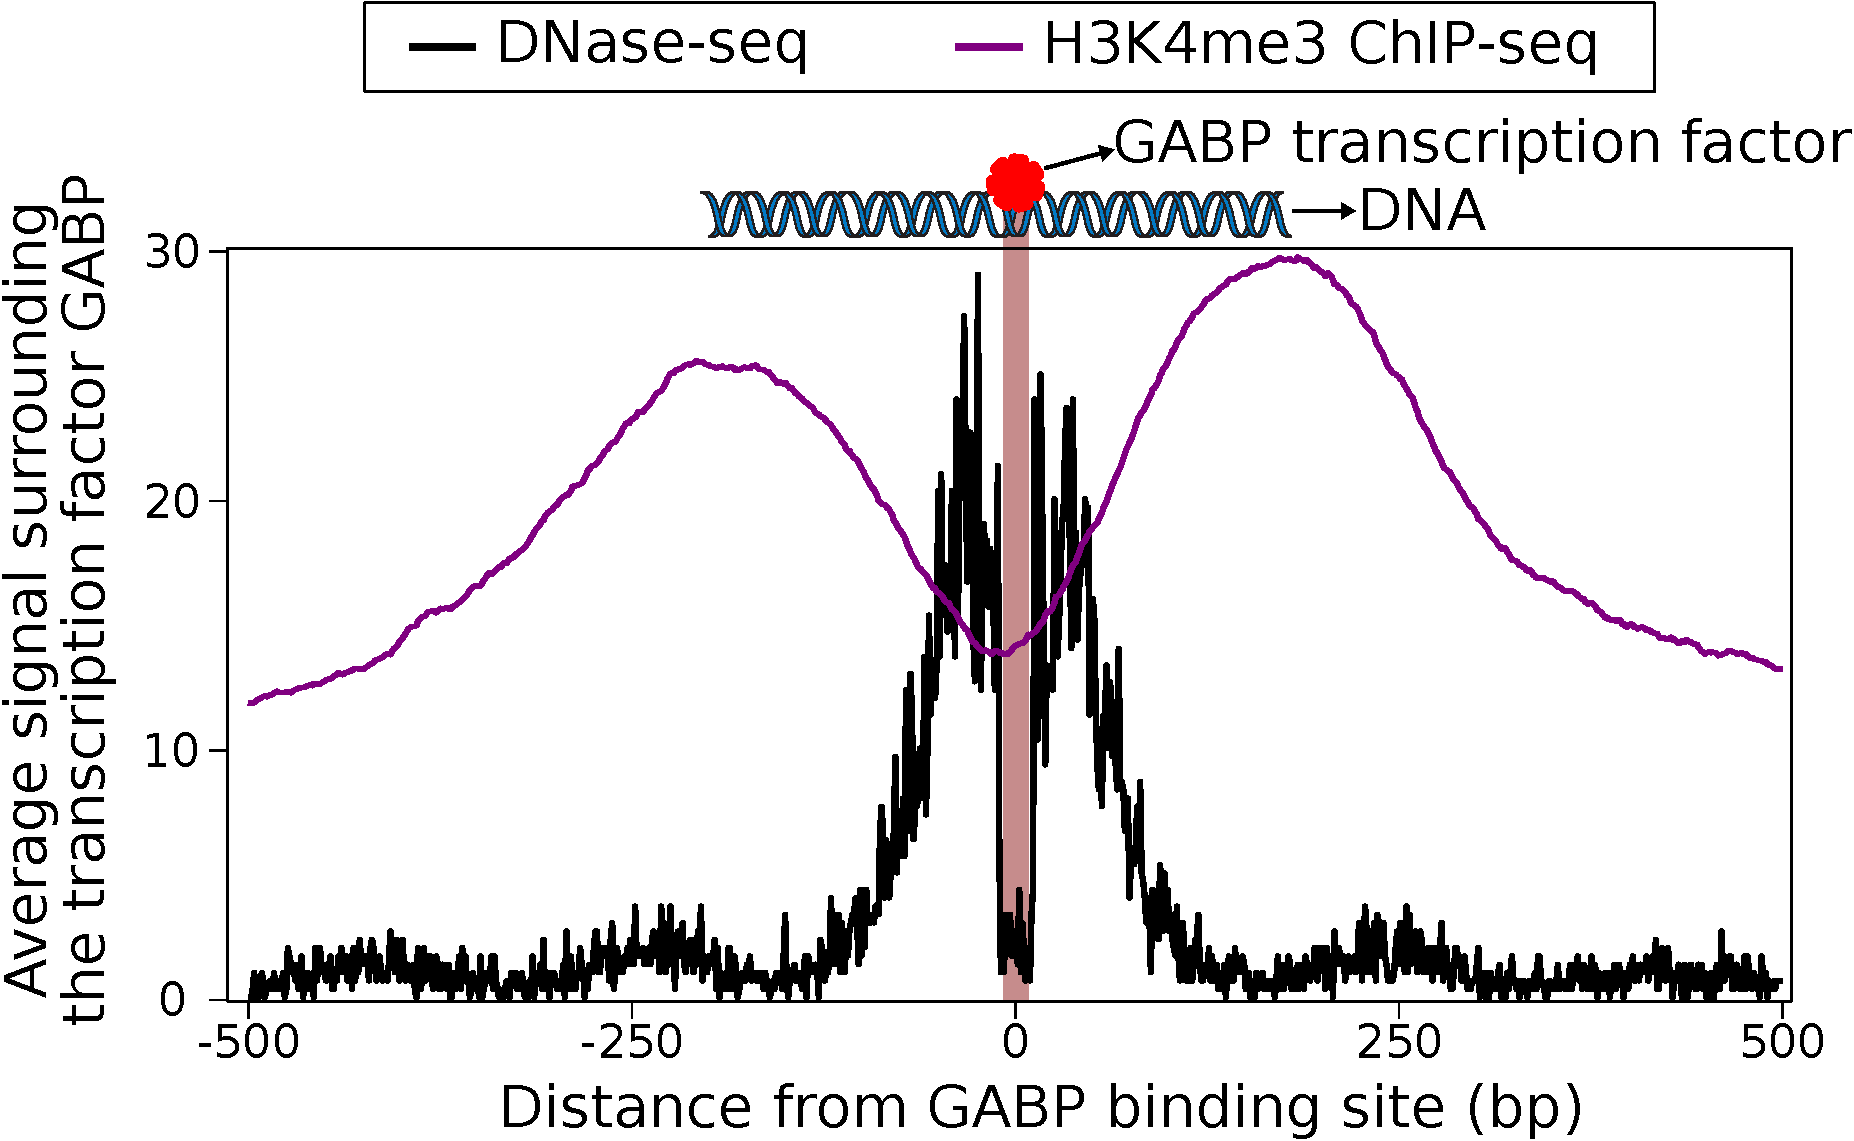
\includegraphics[width=0.8\textwidth]{gusmao_tfbs_pattern}
\caption[Distinctive pattern of DNase-seq and ChIP-seq on active TFBSs]{\textbf{Distinctive pattern of DNase-seq and ChIP-seq on active TFBSs.} In this figure we show the average DNase-seq and histone modification H3K4me3 ChIP-seq signals surrounding the TF GABP active binding sites. Active TFBSs happen at depletions between two peaks of the DNase-seq signal (marked in red). Furthermore, these DNase-seq peaks, which determines an open chromatin region, happen at the depletion between two peaks of active histone modification marks.}
\label{fig:gusmao_tfbs_pattern}
\end{figure}

%%%%%%%%%%%%%%%%%%%%%%%%%%%%%%%%%%%%%%%%%%%%%%%%%%%%%%%%%%%%%%%%%%%%%
% Section: Problem Motivation
%%%%%%%%%%%%%%%%%%%%%%%%%%%%%%%%%%%%%%%%%%%%%%%%%%%%%%%%%%%%%%%%%%%%%
\section{Problem Motivation}
\label{sec:problem.motivation}

% Genome is not enough
A couple of years ago, it was believed that, in possession of the complete genome for a given organism, it would be possible to exactly determine its phenotype and disease susceptibility. However, after the analysis of the first genomes, it was clear that the simple determination of an organism's DNA nucleotide sequence is not enough to explain the great diversity of biological processes. Such processes are governed by a complex chain of events involving regulatory mechanisms, in which genes are turned on (i.e. they are expressed) and off (i.e. they are not expressed) dynamically.

% Gene regulation
These regulatory mechanisms drive the correct execution of biological processes such as development, proliferation, aging, differentiation and many others; and require a set of carefully orchestrated steps that depends on the correct spatial and temporal expression of genes~\citep{maston2006}. Therefore, the deregulation of gene expression is often linked to diseases~\citep{encode2012}. In the so-called post-genomic era, attention is turning to the understanding of how protein-coding genes (about $25,000$ in humans) and their products are regulated~\citep{maston2006}.

% Regulatory elements
To understand the molecular mechanisms that dictate the cell's expression patterns, it is important to identify the regulatory elements involved in these activities. One of the most important regulatory features are transcription factors (TFs) -- proteins that bind on the DNA enhancing or repressing the expression of genes. These proteins bind to particular genomic regions called transcription factor binding sites (TFBSs)~\citep{maston2006}.

% Sequence-based methods
The first computational approach to identify TFBSs was based solely on the DNA sequence~\citep{stormo2000}. Each TF has a particular DNA sequence affinity, i.e. they tend to bind to specific DNA sequences. The computational sequence-based methods search the genome for DNA substrings that corresponds to target TFs. However, computational sequence-based methods are not able to identify \emph{active} TFBSs, i.e. regions in the genome which are currently being bound by a TF~\citep{pique2011}. This happens because such computational approach does not consider the fact that only a few regions in the genome are accessible for TFs to bind. These regions are called ``open chromatin regions''. The number of open chromatin regions and their location vary between different cell types and ultimately dictates which genes are accessible and being expressed~\citep{encode2012}.

% NGS techniques
Nevertheless, advances in DNA sequencing techniques~\citep{shendure2008} have enabled the creation of experimental methods to identify these open chromatin regions and perform more accurate computational prediction of active TFBSs~\citep{encode2012}. We will explore two of these so-called next-generation sequencing (NGS) techniques: the chromatin immunoprecipitation followed by NGS -- termed ChIP-seq~\citep{johnson2007}; and the DNase I cleavage followed by NGS -- termed DNase-seq~\citep{crawford2004,sabo2004a}. These techniques generate signals which span the entire genome and present patterns indicative of open chromatin regions.

% Histone modification ChIP-seq and DNase-seq
The DNA is found wrapped in proteins called histones. There are a number of post-translational modifications on these histones which are indicative of open chromatin regions, such as the so-called H3K4me1 and H3K4me3. By performing a histone modification ChIP-seq experiment we are able to identify cell-specific open chromatin regions. Furthermore, the DNase-seq data also provides a robust map of open chromatin regions with a very high spatial resolution. By combining these two experimental data, we observe very characteristic patterns indicating the active binding of TFs in the genome (see Figure~\ref{fig:gusmao_tfbs_pattern}). This pattern is commonly referred to as TF ``footprints''.

% Computational footprinting methods
The experiments presented in this thesis focus on the computational treatment of DNase-seq and histone modification ChIP-seq data to perform computational predictions of active transcription binding sites. Such prediction is performed by searching the distinctive patterns that the DNase-seq and histone modification ChIP-seq signals exhibit around active TFBSs. We call the computational methods that perform the search for active TFBSs using open chromatin data, such as DNase-seq and histone modification ChIP-seq, ``computational footprinting methods''. The computational footprinting framework presented in this thesis can be used in multiple different biological experiments to understand the regulation of genes.

% Figure - Distinctive pattern of DNase-seq and ChIP-seq on active TFBSs
\begin{figure}[h!]
\centering
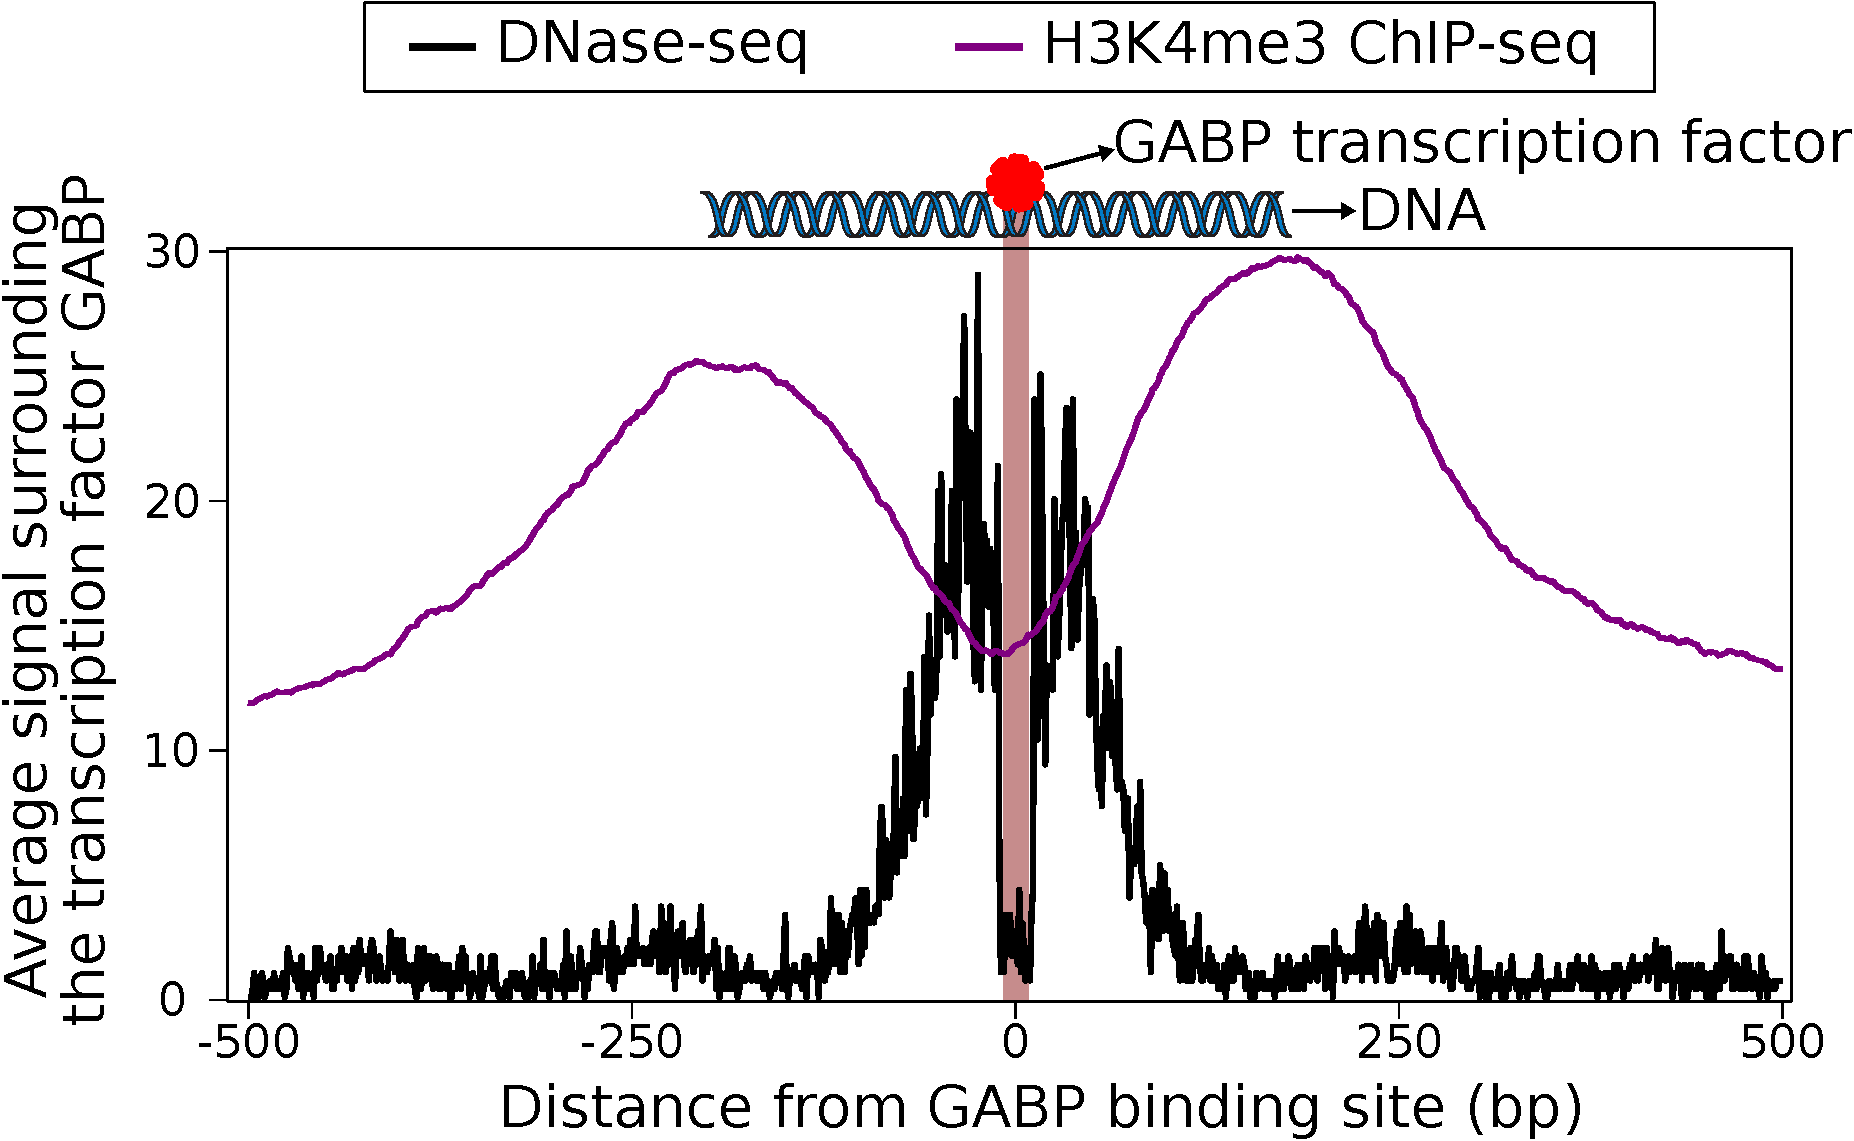
\includegraphics[width=0.8\textwidth]{gusmao_tfbs_pattern}
\caption[Distinctive pattern of DNase-seq and ChIP-seq on active TFBSs]{\textbf{Distinctive pattern of DNase-seq and ChIP-seq on active TFBSs.} In this figure we show the average DNase-seq and histone modification H3K4me3 ChIP-seq signals surrounding the TF GABP active binding sites. Active TFBSs happen at depletions between two peaks of the DNase-seq signal (marked in red). Furthermore, these DNase-seq peaks, which determines an open chromatin region, happen at the depletion between two peaks of active histone modification marks.}
\label{fig:gusmao_tfbs_pattern}
\end{figure}

%%%%%%%%%%%%%%%%%%%%%%%%%%%%%%%%%%%%%%%%%%%%%%%%%%%%%%%%%%%%%%%%%%%%%
% Section: Contributions
%%%%%%%%%%%%%%%%%%%%%%%%%%%%%%%%%%%%%%%%%%%%%%%%%%%%%%%%%%%%%%%%%%%%%
\section{Contributions}
\label{sec:contributions}

% Framework to analyze active TFBSs
The main contribution of this work is the development of a novel computational framework to treat data generated with the DNase-seq and ChIP-seq technologies and detect active TFBSs based on these data. Our contributions are summarized as follows.

% Contributions
\begin{itemize}
  \item \textbf{Novel signal treatment strategy:} Novel DNase-seq and histone modification ChIP-seq signal treatment approaches were developed and formalized. Such treatment framework has shown to be robust and applicable to a wide range of different datasets.
  \item \textbf{DNase-seq experimental bias correction:} We created an approach to correct a known artifact on DNase-seq data -- the DNase-seq sequence cleavage bias. Our experiments have shown the efficiency of such correction on bias mitigation.
  \item \textbf{Novel computational footprinting method:} We devised a novel computational footprinting method based on hidden Markov models (HMMs). It was shown to provide robust active TFBS predictions on the basis of an extensive evaluation process.
  \item \textbf{Novel evaluation of computational footprinting methods:} A novel computational footprinting method evaluation approach based on gene expression was developed. The ranking of methods' accuracies based on this novel evaluation methodology correlated significantly with the methods' ranking for the traditional ChIP-seq evaluation approach.
  \item \textbf{Comprehensive computational footprinting method comparison:} We performed a comprehensive comparison including: (1) our novel HMM-based approach; (2) nine state-of-the-art computational footprinting methods and (3) four baseline approaches. Our comparative experiment is the most complete so far, with a total of $14$ computational footprinting methods and $233$ TFs evaluated.
  \item \textbf{Analysis of relevant features on computational footprinting:} A number of empirical analyses were performed. These analyses evaluated relevant features for the computational prediction of active TFBSs such as: method's parameter selection, experimental bias correction, optimal footprint scoring strategy and TF binding residence time.
  \item \textbf{Case studies:} We successfully applied our computational footprinting method in two different studies to identify regulatory elements involved in specific biological conditions.
\end{itemize}

%%%%%%%%%%%%%%%%%%%%%%%%%%%%%%%%%%%%%%%%%%%%%%%%%%%%%%%%%%%%%%%%%%%%%
% Section: Document Structure
%%%%%%%%%%%%%%%%%%%%%%%%%%%%%%%%%%%%%%%%%%%%%%%%%%%%%%%%%%%%%%%%%%%%%
\section{Document Structure}
\label{sec:document.structure}

% Chapter 2
In Chapter~\ref{cha:background} we introduce all the concepts needed for the understanding of our work. We define the current challenges on computational identification of active TFBSs and provide a comprehensive literature review on computational footprinting methods.

% Chapter 3 / 4
In Chapter~\ref{cha:methods} we formalize our approach to address the detection of active TFBSs. We describe the treatment of the input DNase-seq and ChIP-seq data and the novel approach to detect active TFBSs based on HMMs. Furthermore, in Chapter~\ref{cha:experiments} we describe the full experiment design of this project. We present: the data used in our work, the execution of our computational footprinting approach and the method evaluation strategies.

% Chapter 5 / 6
In Chapter~\ref{cha:results} we present the results of our experiments, which encompasses: the analyses on relevant computational footprinting features, a comprehensive comparison of computational footprinting methods and case studies in which our methodology was successfully applied to real biological scenarios. In Chapter~\ref{cha:conclusion} we discuss all results presented in this thesis, highlighting all the key findings. Furthermore, we discuss future research opportunities. Further supplementary results, figures and tables can be found in the Appendix~\ref{cha:appendix}.






%%%%%%%%%%%%%%%%%%%%%%%%%%%%%%%%%%%%%%%%%%%%%%%%%%%%%%%%%%%%%%%%%%%%%%%%%%%%%%%%%%%%%%%%%%%%%%%%%%%
% Chapter 1 -> Introduction
% Author: Eduardo G Gusmao
%%%%%%%%%%%%%%%%%%%%%%%%%%%%%%%%%%%%%%%%%%%%%%%%%%%%%%%%%%%%%%%%%%%%%%%%%%%%%%%%%%%%%%%%%%%%%%%%%%%
\chapter{Introduction}
\label{cha:introduction}

\graphicspath{{chapter1/figs/}}

%%%%%%%%%%%%%%%%%%%%%%%%%%%%%%%%%%%%%%%%%%%%%%%%%%%%%%%%%%%%%%%%%%%%%
% Section: Motivation
%%%%%%%%%%%%%%%%%%%%%%%%%%%%%%%%%%%%%%%%%%%%%%%%%%%%%%%%%%%%%%%%%%%%%
\section{Motivation}
\label{sec:problem.motivation}

\subsubsection{Gene Regulation}

Every living organism is composed of multiple different cells. These cells contain genetic material encoded in the form of DNA molecules, also known as genome. The genome can be represented as a categorical vector $\mathbf{g} = \langle g_1, ..., g_n \rangle$, where $g_i \in \{\text{A},\text{C},\text{G},\text{T}\}$ represents the nucleotide at genomic position $i$. Certain substrings of the genome $\mathbf{g}$, denoted as $\mathbf{g}[u..v]$, from genomic positions $u$ to $v$ for $u < v \leq n$, represent genes. Genes can be read by specialized proteins to produce other proteins. This protein-producing cycle is the key mechanism for life mantainance.

Nevertheless, the genomic sequence $\mathbf{g}$ is the same for all different cell types that compose a multicellular organism, such as the human. The great difference observed by different cell types is achieved by selectivelly turning some genes ``on'' and ``off''. This process is known as gene regulation. 

\subsubsection{Transcription Factor Binding Sites}



\subsubsection{Importance of the Identification of Active TFBSs}




\subsubsection{Computational Detection of Active TFBSs Must Consider the Chromatin Dynamics}



\subsubsection{Distinctive Patterns in DNase-seq and ChIP-seq Signals Shape Active TFBSs}


%%%%%%%%%%%%%%%%%%%%%%%%%%%%%%%%%%%%%%%%%%%%%%%%%%%%%%%%%%%%%%%%%%%%%
% Section: Contributions
%%%%%%%%%%%%%%%%%%%%%%%%%%%%%%%%%%%%%%%%%%%%%%%%%%%%%%%%%%%%%%%%%%%%%
\section{Contributions}
\label{sec:contributions}

% Framework to analyze active TFBSs
The main contribution of this work is the development of a novel computational framework to treat data generated with the DNase-seq and ChIP-seq technologies and detect active TFBSs based on these data. Our contributions are summarized as follows.

% Contributions
\begin{itemize}
  \item \textbf{Novel signal treatment strategy:} Novel DNase-seq and histone modification ChIP-seq signal treatment approaches were developed and formalized. Such treatment framework has shown to be robust and applicable to a wide range of different datasets.
  \item \textbf{DNase-seq experimental bias correction:} We created an approach to correct for known artifacts on DNase-seq data generated by the DNase-seq sequence cleavage bias. Our experiments have shown the efficiency of such correction on bias mitigation.
  \item \textbf{Novel computational footprinting method:} We devised a novel computational footprinting method based on hidden Markov models (HMMs). It was shown to provide robust active TFBS predictions on the basis of an extensive evaluation process.
  \item \textbf{Novel evaluation of computational footprinting methods:} A novel computational footprinting method evaluation approach based on gene expression was developed. The ranking of methods' accuracies based on this novel evaluation methodology correlated significantly with the methods' ranking for the traditional ChIP-seq evaluation approach.
  \item \textbf{Comprehensive computational footprinting method comparison:} We performed a comprehensive comparison including: (1) our novel HMM-based approach; (2) nine state-of-the-art computational footprinting methods and (3) four baseline approaches. Our comparative experiment is the most complete so far, with a total of $14$ computational footprinting methods and $233$ TFs evaluated.
  \item \textbf{Analysis of relevant features on computational footprinting:} A number of empirical analyses were performed. These analyses evaluated relevant features for the computational prediction of active TFBSs such as: method's parameter selection, experimental bias correction, optimal footprint scoring strategy and TF binding residence time.
  \item \textbf{Case studies:} We successfully applied our computational footprinting method in two different studies to identify regulatory elements involved in specific biological conditions.
\end{itemize}

%%%%%%%%%%%%%%%%%%%%%%%%%%%%%%%%%%%%%%%%%%%%%%%%%%%%%%%%%%%%%%%%%%%%%
% Section: Document Structure
%%%%%%%%%%%%%%%%%%%%%%%%%%%%%%%%%%%%%%%%%%%%%%%%%%%%%%%%%%%%%%%%%%%%%
\section{Document Structure}
\label{sec:document.structure}

% Chapter 2
In Chapter~\ref{cha:background} we introduce all the concepts needed for the understanding of our work. We define the current challenges on computational identification of active TFBSs and provide a comprehensive literature review on computational footprinting methods.

% Chapter 3 / 4
In Chapter~\ref{cha:methods} we formalize our approach to address the detection of active TFBSs. We describe the treatment of the input DNase-seq and ChIP-seq data and the novel approach to detect active TFBSs based on HMMs. Furthermore, in Chapter~\ref{cha:experiments} we describe the full experiment design of this project. We present: the data used in our work, the execution of our computational footprinting approach and the method evaluation strategies.

% Chapter 5 / 6
In Chapter~\ref{cha:results} we present the results of our experiments, which encompasses: the analyses on relevant computational footprinting features, a comprehensive comparison of computational footprinting methods and case studies in which our methodology was successfully applied to real biological scenarios. In Chapter~\ref{cha:conclusion} we discuss all results presented in this thesis, highlighting all the key findings. Furthermore, we discuss future research opportunities. Further supplementary results, figures and tables can be found in the Appendix~\ref{cha:appendix}.



